\chapter{Loss, Optimization, And Learning}

A GPT model learns by being wrong in a measurable way. The forward pass produces logits. The loss function turns logits and targets into one scalar number. Backpropagation turns that scalar into gradients. The optimizer turns gradients into parameter updates. Repeating this process many times is training.

This chapter connects the mathematical idea of learning to the exact engineering loop used by TinyGPT.

\section{Chapter Goals}

By the end of this chapter, you should be able to:

\begin{itemize}
  \item convert logits into probabilities with softmax;
  \item compute cross-entropy loss for one TinyGPT prediction;
  \item explain why the correct token receives a different gradient signal from incorrect tokens;
  \item describe how gradients flow backward through the model;
  \item distinguish parameters, gradients, optimizer state, and activations;
  \item explain SGD, AdamW, weight decay, learning-rate schedules, gradient clipping, and gradient accumulation;
  \item read a complete training loop and understand why each line is ordered that way;
  \item diagnose common loss-curve behaviors during training.
\end{itemize}

\section{The Training Step In One Picture}

At a high level, one training step looks like this:

\begin{center}
\resizebox{\textwidth}{!}{
\begin{tikzpicture}[
  box/.style={draw, rounded corners=2pt, minimum height=0.66cm, text width=2.15cm, align=center},
  arrow/.style={-{Latex[length=2mm]}, thick},
  back/.style={{Latex[length=2mm]}-, thick, red!70!black},
  note/.style={font=\small, align=center}
]
\node[box, fill=blue!5] (batch) at (0,0) {batch\\\(x,y\)};
\node[box, fill=red!8] (model) at (2.8,0) {TinyGPT\\\(f_\theta\)};
\node[box, fill=green!10] (logits) at (5.6,0) {logits\\\shape{[B,T,V]}};
\node[box, fill=yellow!18] (loss) at (8.4,0) {loss\\scalar};
\node[box, fill=gray!12] (grads) at (5.6,-1.35) {gradients\\\(\nabla_\theta L\)};
\node[box, fill=gray!12] (opt) at (2.8,-1.35) {optimizer\\AdamW};
\draw[arrow] (batch) -- (model);
\draw[arrow] (model) -- (logits);
\draw[arrow] (logits) -- (loss);
\draw[arrow] (loss) -- (grads);
\draw[arrow] (grads) -- (opt);
\draw[arrow] (opt) -- (model);
\node[note] at (5.6,-2.25) {Forward computes loss. Backward computes gradients. Optimizer updates parameters.};
\end{tikzpicture}}
\end{center}

The parameter vector \(\theta\) changes only during the optimizer step. The input batch does not learn. The activations are temporary. The gradients are temporary. The optimizer state persists across steps.

\section{The Running TinyGPT Prediction}

Suppose TinyGPT sees:

\begin{quote}
\texttt{Tiny GPT models learn from}
\end{quote}

and the correct next token is:

\begin{quote}
\texttt{tokens}
\end{quote}

In our toy vocabulary:

\[
\texttt{tokens}=7.
\]

The model outputs one logit per vocabulary token:

\[
\mathbf{z}=
\begin{bmatrix}
z_0&z_1&z_2&z_3&z_4&z_5&z_6&z_7&z_8
\end{bmatrix}.
\]

Example logits:

\[
\mathbf{z}=
\begin{bmatrix}
-1.0&-0.8&0.1&0.2&0.0&0.5&0.3&1.7&-0.4
\end{bmatrix}.
\]

\begin{center}
\resizebox{0.96\textwidth}{!}{
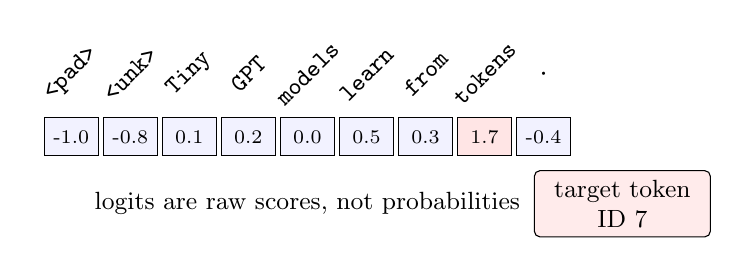
\begin{tikzpicture}[
  cell/.style={draw, minimum width=0.68cm, minimum height=0.48cm, align=center},
  note/.style={font=\small, align=center},
  arrow/.style={-{Latex[length=2mm]}, thick}
]
\foreach \i/\tok in {0/<pad>,1/<unk>,2/Tiny,3/GPT,4/models,5/learn,6/from,7/tokens,8/.} {
  \node[note, rotate=45] at (\i*0.75,0.8) {\texttt{\tok}};
}
\foreach \i/\v in {0/-1.0,1/-0.8,2/0.1,3/0.2,4/0.0,5/0.5,6/0.3,7/1.7,8/-0.4} {
  \ifnum\i=7
    \node[cell, fill=red!10] at (\i*0.75,0) {\scriptsize \v};
  \else
    \node[cell, fill=blue!5] at (\i*0.75,0) {\scriptsize \v};
  \fi
}
\node[note] at (3.0,-0.85) {logits are raw scores, not probabilities};
\node[note, fill=red!8, draw, rounded corners=2pt, text width=2.0cm] at (7.0,-0.85) {target token\\ID 7};
\end{tikzpicture}}
\end{center}

A logit can be any real number. Higher means the model prefers that token more, but logits are not probabilities until softmax is applied.

\section{Softmax: Scores Become Probabilities}

Softmax converts logits into a probability distribution:

\[
p_i=\frac{e^{z_i}}{\sum_{j=0}^{V-1}e^{z_j}}.
\]

The probabilities satisfy:

\[
p_i\geq0,\qquad \sum_i p_i=1.
\]

\begin{center}
\resizebox{0.92\textwidth}{!}{
\begin{tikzpicture}[
  cell/.style={draw, minimum width=0.62cm, minimum height=0.48cm, align=center},
  box/.style={draw, rounded corners=2pt, minimum height=0.66cm, text width=1.8cm, align=center},
  arrow/.style={-{Latex[length=2mm]}, thick},
  note/.style={font=\small, align=center}
]
\foreach \i/\v in {0/-1.0,1/-0.8,2/0.1,3/0.2,4/0.0,5/0.5,6/0.3,7/1.7,8/-0.4} {
  \node[cell, fill=blue!5] at (\i*0.58,0) {\scriptsize \v};
}
\node[note] at (2.35,0.65) {logits};
\node[box, fill=yellow!18] (soft) at (6.3,0) {softmax};
\foreach \i/\v in {0/.03,1/.04,2/.09,3/.10,4/.08,5/.13,6/.11,7/.38,8/.05} {
  \ifnum\i=7
    \node[cell, fill=red!10] at (8.0+\i*0.58,0) {\scriptsize \v};
  \else
    \node[cell, fill=green!10] at (8.0+\i*0.58,0) {\scriptsize \v};
  \fi
}
\node[note] at (10.35,0.65) {probabilities};
\draw[arrow] (5.35,0) -- (soft);
\draw[arrow] (soft) -- (7.45,0);
\node[note] at (10.35,-0.8) {probability for correct token ID 7 is \(p_7\approx0.38\)};
\end{tikzpicture}}
\end{center}

In actual code, PyTorch's cross-entropy function combines log-softmax and negative log-likelihood in a numerically stable way. We usually do not call softmax manually during training.

\section{Cross Entropy For One Prediction}

If the correct token is \(y=7\), the loss for one prediction is:

\[
\ell=-\log p_y=-\log p_7.
\]

If \(p_7=0.38\):

\[
\ell=-\log(0.38)\approx0.97.
\]

If \(p_7=0.05\):

\[
\ell=-\log(0.05)\approx3.00.
\]

If \(p_7=0.90\):

\[
\ell=-\log(0.90)\approx0.105.
\]

\begin{center}
\begin{tikzpicture}[
  box/.style={draw, rounded corners=2pt, minimum height=0.65cm, text width=2.2cm, align=center},
  arrow/.style={-{Latex[length=2mm]}, thick}
]
\node[box, fill=red!8] (bad) at (0,0) {\(p_y=0.05\)\\loss \(3.00\)};
\node[box, fill=yellow!18] (mid) at (3.2,0) {\(p_y=0.38\)\\loss \(0.97\)};
\node[box, fill=green!10] (good) at (6.4,0) {\(p_y=0.90\)\\loss \(0.105\)};
\draw[arrow] (bad) -- node[above, font=\small] {better model} (mid);
\draw[arrow] (mid) -- node[above, font=\small] {better model} (good);
\end{tikzpicture}
\end{center}

Cross entropy strongly punishes the model when it gives low probability to the correct token.

\section{Batch Loss}

TinyGPT predicts the next token at every position in every example. For logits:

\[
Z\in\mathbb{R}^{B\times T\times V}
\]

and targets:

\[
y\in\mathbb{Z}^{B\times T},
\]

the batch loss is:

\[
L=\frac{1}{BT}\sum_{b=1}^{B}\sum_{t=1}^{T}-\log p_{b,t,y_{b,t}}.
\]

\begin{center}
\resizebox{0.96\textwidth}{!}{
\begin{tikzpicture}[
  cell/.style={draw, minimum width=0.55cm, minimum height=0.45cm, align=center},
  box/.style={draw, rounded corners=2pt, minimum height=0.66cm, text width=1.9cm, align=center},
  arrow/.style={-{Latex[length=2mm]}, thick},
  note/.style={font=\small, align=center}
]
\node[note] at (1.4,0.65) {8 position losses\\\(B=2,T=4\)};
\foreach \r in {0,1} {
  \foreach \c/\v in {0/1.2,1/0.8,2/1.5,3/0.9} {
    \node[cell, fill=yellow!18] at (\c*0.65,-\r*0.5) {\scriptsize \v};
  }
}
\node[box, fill=red!8] (mean) at (4.2,-0.25) {mean};
\node[box, fill=green!10] (loss) at (7.0,-0.25) {batch loss\\scalar};
\draw[arrow] (2.8,-0.25) -- (mean);
\draw[arrow] (mean) -- (loss);
\node[note] at (3.5,-1.25) {Training usually optimizes the average loss per predicted token.};
\end{tikzpicture}}
\end{center}

The loss is a scalar so that gradient descent has one objective to reduce.

\section{The Gradient Signal}

For one prediction, softmax plus cross entropy has a useful derivative:

\[
\frac{\partial \ell}{\partial z_i}=p_i-\mathbb{1}[i=y].
\]

This means:

\begin{itemize}
  \item for the correct token \(i=y\), the gradient is \(p_y-1\), usually negative;
  \item for an incorrect token \(i\neq y\), the gradient is \(p_i\), positive;
  \item the model is pushed to raise the correct logit and lower incorrect logits.
\end{itemize}

\begin{center}
\resizebox{0.95\textwidth}{!}{
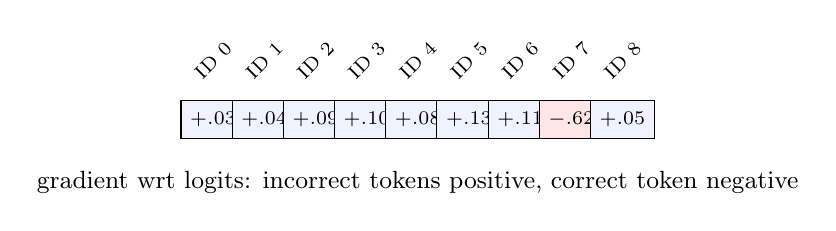
\begin{tikzpicture}[
  cell/.style={draw, minimum width=0.62cm, minimum height=0.48cm, align=center},
  note/.style={font=\small, align=center}
]
\foreach \i/\p in {0/.03,1/.04,2/.09,3/.10,4/.08,5/.13,6/.11,7/.38,8/.05} {
  \node[note, rotate=45] at (\i*0.65,0.75) {\scriptsize ID \i};
  \ifnum\i=7
    \node[cell, fill=red!10] at (\i*0.65,0) {\scriptsize \(-.62\)};
  \else
    \node[cell, fill=blue!5] at (\i*0.65,0) {\scriptsize \(+\p\)};
  \fi
}
\node[note] at (2.6,-0.8) {gradient wrt logits: incorrect tokens positive, correct token negative};
\end{tikzpicture}}
\end{center}

During gradient descent:

\[
\theta \leftarrow \theta-\eta\nabla_\theta L.
\]

A negative gradient on the correct logit means the update tends to increase that logit next time.

\section{Backpropagation: Gradients Flow Through The Whole Model}

The loss is computed at the output, but it affects every trainable parameter that contributed to the logits:

\[
L \rightarrow W_{\text{out}} \rightarrow X_N \rightarrow \cdots \rightarrow E_{\text{tok}}.
\]

\begin{center}
\resizebox{\textwidth}{!}{
\begin{tikzpicture}[
  box/.style={draw, rounded corners=2pt, minimum height=0.62cm, text width=1.85cm, align=center},
  arrow/.style={-{Latex[length=2mm]}, thick},
  back/.style={{Latex[length=2mm]}-, thick, red!70!black},
  note/.style={font=\small, align=center}
]
\node[box, fill=blue!5, font=\small] (emb) at (0,0) {embeddings};
\node[box, fill=red!8] (b1) at (2.2,0) {block 1};
\node[box, fill=red!8] (b2) at (4.4,0) {block 2};
\node[box, fill=yellow!18] (ln) at (6.6,0) {final LN};
\node[box, fill=green!10] (head) at (8.8,0) {LM head};
\node[box, fill=gray!12] (loss) at (11.0,0) {loss};
\draw[arrow] (emb) -- (b1);
\draw[arrow] (b1) -- (b2);
\draw[arrow] (b2) -- (ln);
\draw[arrow] (ln) -- (head);
\draw[arrow] (head) -- (loss);
\draw[back] (emb.south) .. controls (3,-1.4) and (8,-1.4) .. (loss.south);
\node[note] at (5.5,-1.8) {Backpropagation applies the chain rule through every differentiable operation.};
\end{tikzpicture}}
\end{center}

Autograd stores enough information from the forward pass to compute gradients. This is why training uses more memory than inference.

\section{Parameters, Gradients, And Optimizer State}

It is important to separate four kinds of tensors:

\begin{longtable}{p{0.22\textwidth}p{0.24\textwidth}p{0.38\textwidth}}
\toprule
\term{Tensor kind} & \term{Example} & \term{Role} \\
\midrule
Parameter & embedding weights & trainable model memory \\
Activation & hidden state \(X_\ell\) & temporary forward-pass value \\
Gradient & \texttt{weight.grad} & direction for parameter update \\
Optimizer state & AdamW moments & persistent update history \\
\bottomrule
\end{longtable}

\begin{center}
\begin{tikzpicture}[
  box/.style={draw, rounded corners=2pt, minimum height=0.65cm, text width=2.4cm, align=center},
  arrow/.style={-{Latex[length=2mm]}, thick}
]
\node[box, fill=blue!5] (param) at (0,0) {parameter\\\(\theta\)};
\node[box, fill=yellow!18] (grad) at (3,0) {gradient\\\(g_t\)};
\node[box, fill=gray!12] (state) at (6,0.8) {AdamW state\\\(m_t,v_t\)};
\node[box, fill=red!8] (new) at (6,-0.8) {updated parameter\\\(\theta_{t+1}\)};
\draw[arrow] (param) -- (grad);
\draw[arrow] (grad) -- (state);
\draw[arrow] (grad) -- (new);
\draw[arrow] (state) -- (new);
\end{tikzpicture}
\end{center}

When resuming training, optimizer state matters. If it is missing, training can still continue, but the optimizer has lost its momentum/history.

\section{Plain Gradient Descent}

The simplest update is:

\[
\theta_{t+1}=\theta_t-\eta g_t,
\]

where:

\[
g_t=\nabla_\theta L(\theta_t).
\]

The learning rate \(\eta\) controls step size.

\begin{center}
\begin{tikzpicture}[
  arrow/.style={-{Latex[length=2mm]}, thick},
  note/.style={font=\small, align=center}
]
\draw[->] (-0.2,0) -- (6.5,0) node[right] {\scriptsize parameter};
\draw[->] (0,-0.2) -- (0,3) node[above] {\scriptsize loss};
\draw[thick, blue!70!black] plot[smooth] coordinates {(0.3,2.6) (1.2,1.6) (2.5,0.7) (3.8,1.0) (5.5,2.2)};
\filldraw[red!70!black] (1.2,1.6) circle (2pt);
\draw[arrow, red!70!black] (1.2,1.6) -- (1.95,1.05);
\node[note] at (2.4,1.55) {step opposite\\the gradient};
\node[note] at (3.2,-0.45) {Training searches for parameters with lower loss.};
\end{tikzpicture}
\end{center}

Plain gradient descent is useful for understanding, but modern GPTs usually use AdamW.

\section{AdamW}

AdamW tracks moving averages of gradients and squared gradients:

\[
m_t=\beta_1m_{t-1}+(1-\beta_1)g_t,
\]

\[
v_t=\beta_2v_{t-1}+(1-\beta_2)g_t^2.
\]

Intuition:

\begin{itemize}
  \item \(m_t\) is a smoothed direction, like momentum;
  \item \(v_t\) estimates recent gradient scale;
  \item the update normalizes by gradient scale so each parameter has an adaptive step;
  \item decoupled weight decay gently shrinks weights separately from the loss gradient.
\end{itemize}

\begin{center}
\resizebox{0.92\textwidth}{!}{
\begin{tikzpicture}[
  box/.style={draw, rounded corners=2pt, minimum height=0.65cm, text width=2.2cm, align=center},
  arrow/.style={-{Latex[length=2mm]}, thick},
  note/.style={font=\small, align=center}
]
\node[box, fill=blue!5] (g) at (0,0) {gradient\\\(g_t\)};
\node[box, fill=yellow!18] (m) at (3,0.75) {1st moment\\\(m_t\)};
\node[box, fill=yellow!18] (v) at (3,-0.75) {2nd moment\\\(v_t\)};
\node[box, fill=red!8] (upd) at (6,0) {adaptive\\update};
\node[box, fill=green!10] (theta) at (9,0) {new weights\\\(\theta_{t+1}\)};
\draw[arrow] (g) -- (m);
\draw[arrow] (g) -- (v);
\draw[arrow] (m) -- (upd);
\draw[arrow] (v) -- (upd);
\draw[arrow] (upd) -- (theta);
\node[note] at (4.5,-1.55) {AdamW uses both direction and scale history.};
\end{tikzpicture}}
\end{center}

Typical GPT-style values:

\begin{lstlisting}
optimizer = torch.optim.AdamW(
    model.parameters(),
    lr=learning_rate,
    betas=(0.9, 0.95),
    weight_decay=0.1,
)
\end{lstlisting}

Hyperparameters are not universal laws. They should be recorded in config and logs.

\section{Learning Rate Schedules}

The learning rate controls how far the optimizer moves each step. A common GPT schedule uses warmup followed by cosine decay:

\[
\eta(s)=
\begin{cases}
\eta_{\max}\dfrac{s}{s_{\text{warmup}}}, & s<s_{\text{warmup}},\\
\eta_{\min}
+\dfrac{1}{2}(\eta_{\max}-\eta_{\min})
\left(1+\cos\left(\pi\dfrac{s-s_{\text{warmup}}}{s_{\text{total}}-s_{\text{warmup}}}\right)\right),
& s\geq s_{\text{warmup}}.
\end{cases}
\]

\begin{center}
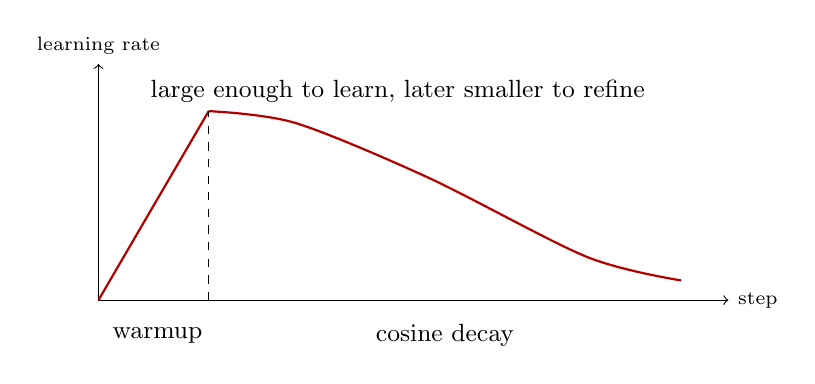
\begin{tikzpicture}[
  note/.style={font=\small, align=center}
]
\draw[->] (0,0) -- (8,0) node[right] {\scriptsize step};
\draw[->] (0,0) -- (0,3) node[above] {\scriptsize learning rate};
\draw[thick, red!70!black] (0,0) -- (1.4,2.4);
\draw[thick, red!70!black] plot[smooth] coordinates {(1.4,2.4) (2.5,2.25) (4.2,1.55) (6.2,0.55) (7.4,0.25)};
\draw[dashed] (1.4,0) -- (1.4,2.4);
\node[note] at (0.75,-0.45) {warmup};
\node[note] at (4.4,-0.45) {cosine decay};
\node[note] at (3.8,2.65) {large enough to learn, later smaller to refine};
\end{tikzpicture}
\end{center}

Warmup prevents unstable early updates when weights are random and gradients can be noisy. Decay allows smaller, more careful updates later.

\section{Gradient Accumulation}

If GPU memory cannot fit a large batch, we can split it into microbatches and accumulate gradients:

\[
B_{\text{effective}}
=B_{\text{micro}}\times \texttt{grad\_accum\_steps}\times \texttt{world\_size}.
\]

\begin{center}
\resizebox{0.96\textwidth}{!}{
\begin{tikzpicture}[
  box/.style={draw, rounded corners=2pt, minimum height=0.62cm, text width=2.0cm, align=center},
  arrow/.style={-{Latex[length=2mm]}, thick},
  note/.style={font=\small, align=center}
]
\node[box, fill=blue!5] (m1) at (0,0) {microbatch 1\\backward};
\node[box, fill=blue!5] (m2) at (2.5,0) {microbatch 2\\backward};
\node[box, fill=blue!5] (m3) at (5.0,0) {microbatch 3\\backward};
\node[box, fill=yellow!18, font=\small] (acc) at (7.5,0) {accumulated\\gradients};
\node[box, fill=red!8] (step) at (10.0,0) {one optimizer\\step};
\draw[arrow] (m1) -- (m2);
\draw[arrow] (m2) -- (m3);
\draw[arrow] (m3) -- (acc);
\draw[arrow] (acc) -- (step);
\node[note] at (5,-0.9) {Scale each microbatch loss by \(1/\texttt{grad\_accum\_steps}\).};
\end{tikzpicture}}
\end{center}

Code pattern:

\begin{lstlisting}[language=Python]
optimizer.zero_grad(set_to_none=True)

for micro_step in range(grad_accum_steps):
    x, y = get_batch()
    logits, loss = model(x, y)
    loss = loss / grad_accum_steps
    loss.backward()

torch.nn.utils.clip_grad_norm_(model.parameters(), max_norm)
optimizer.step()
\end{lstlisting}

Dividing the loss keeps the accumulated gradient scale comparable to one large batch.

\section{Gradient Clipping}

Gradient clipping limits rare extreme updates:

\[
g\leftarrow g\cdot \min\left(1,\frac{c}{\|g\|}\right).
\]

If \(\|g\|\leq c\), nothing changes. If \(\|g\|>c\), the gradient is scaled down.

\begin{center}
\begin{tikzpicture}[
  arrow/.style={-{Latex[length=2mm]}, thick},
  note/.style={font=\small, align=center}
]
\draw[->] (0,0) -- (5.5,0) node[right] {\scriptsize gradient direction};
\draw[arrow, red!70!black] (0,0.9) -- (5.0,0.9);
\node[note] at (2.5,1.35) {too large};
\draw[arrow, green!60!black] (0,-0.4) -- (2.6,-0.4);
\node[note] at (1.3,-0.85) {clipped norm};
\draw[dashed] (2.6,-1.1) -- (2.6,1.5);
\node[note] at (2.9,-1.25) {max norm \(c\)};
\end{tikzpicture}
\end{center}

Clipping does not fix a broken training setup, but it can prevent occasional spikes from damaging training.

\section{The Full Training Loop}

A practical TinyGPT training loop:

\begin{lstlisting}[language=Python]
for step in range(max_steps):
    model.train()
    optimizer.zero_grad(set_to_none=True)

    for micro_step in range(grad_accum_steps):
        x, y = get_batch("train")
        logits, loss = model(x, y)
        (loss / grad_accum_steps).backward()

    grad_norm = torch.nn.utils.clip_grad_norm_(model.parameters(), max_norm)

    lr = get_lr(step)
    for group in optimizer.param_groups:
        group["lr"] = lr

    optimizer.step()

    if step % eval_interval == 0:
        model.eval()
        val_loss = estimate_loss("val")
        log(step, loss.item(), val_loss, lr, grad_norm)
\end{lstlisting}

\begin{center}
\resizebox{\textwidth}{!}{
\begin{tikzpicture}[
  box/.style={draw, rounded corners=2pt, minimum height=0.62cm, text width=1.9cm, align=center},
  arrow/.style={-{Latex[length=2mm]}, thick}
]
\node[box, fill=blue!5] (batch) at (0,0) {get batch};
\node[box, fill=red!8] (forward) at (2.3,0) {forward};
\node[box, fill=yellow!18] (backward) at (4.6,0) {backward};
\node[box, fill=gray!12] (clip) at (6.9,0) {clip};
\node[box, fill=green!10] (step) at (9.2,0) {optimizer\\step};
\node[box, fill=blue!5] (eval) at (11.5,0) {eval/log};
\draw[arrow] (batch) -- (forward);
\draw[arrow] (forward) -- (backward);
\draw[arrow] (backward) -- (clip);
\draw[arrow] (clip) -- (step);
\draw[arrow] (step) -- (eval);
\draw[arrow] (eval) .. controls (6,-1.5) and (2,-1.5) .. (batch);
\end{tikzpicture}}
\end{center}

Order matters. Calling \texttt{optimizer.step()} before \texttt{loss.backward()} would update with missing or stale gradients. Forgetting \texttt{zero\_grad()} would mix gradients from different steps.

\section{The Same Learning Step In Three Backends}

One way this book can be more useful than a single-framework tutorial is to separate the
\emph{mathematics of learning} from the \emph{engineering system that executes it}.
PyTorch, Candle, and llm.c look very different on the surface, but a correct GPT training
step must obey the same contract:

\[
\begin{aligned}
X, Y &\in \mathbb{N}^{B \times T},\\
H &= f_\theta(X),\\
\text{logits} &= H W_{\text{vocab}} + b_{\text{vocab}},\\
\mathcal{L}(\theta) &=
-\frac{1}{BT}\sum_{b=1}^{B}\sum_{t=1}^{T}
\log
\frac{\exp(\text{logits}_{b,t,Y_{b,t}})}
{\sum_{v=1}^{V}\exp(\text{logits}_{b,t,v})},\\
\theta_{k+1} &= \operatorname{AdamW}(\theta_k,\nabla_\theta \mathcal{L}).
\end{aligned}
\]

This is the invariant learning step. The backend is the machinery that stores tensors,
launches kernels, records or computes gradients, and updates weights.

\begin{figure}[htbp]
\centering
\resizebox{\textwidth}{!}{%
\begin{tikzpicture}[
    node distance=1.5cm,
    box/.style={draw, rounded corners, fill=blue!6, minimum width=3.1cm, minimum height=0.85cm, align=center},
    sys/.style={draw, rounded corners, fill=orange!12, minimum width=3.4cm, minimum height=1.05cm, align=center},
    test/.style={draw, rounded corners, fill=green!10, minimum width=3.2cm, minimum height=0.85cm, align=center},
    arrow/.style={-{Latex[length=3mm]}, thick}
]
\node[box] (math) {Backend-invariant\\training math};
\node[sys, below left=1.3cm and 3.4cm of math] (torch) {PyTorch\\autograd reference};
\node[sys, below=1.3cm of math] (candle) {Candle/Rust\\typed systems path};
\node[sys, below right=1.3cm and 3.4cm of math] (llmc) {llm.c/CUDA\\explicit kernel path};
\node[test, below=1.6cm of candle] (checks) {Shared checks:\\loss, samples, checkpoint, throughput};
\draw[arrow] (math) -- (torch);
\draw[arrow] (math) -- (candle);
\draw[arrow] (math) -- (llmc);
\draw[arrow] (torch) -- (checks);
\draw[arrow] (candle) -- (checks);
\draw[arrow] (llmc) -- (checks);
\end{tikzpicture}}
\caption{The three training backends should implement the same mathematical contract, then report comparable evidence.}
\end{figure}

\subsection{PyTorch: The Readable Reference}

The PyTorch path is the first backend because it is the most transparent for learning.
The source code usually looks close to the mathematical graph:

\begin{lstlisting}[language=Python]
logits, loss = model(x, y)
optimizer.zero_grad(set_to_none=True)
loss.backward()
torch.nn.utils.clip_grad_norm_(model.parameters(), max_norm)
optimizer.step()
\end{lstlisting}

The important hidden service is autograd. During the forward pass, PyTorch records a
dynamic computation graph. Every tensor operation that needs gradients stores enough
information for its backward rule. When \texttt{loss.backward()} runs, PyTorch walks that
graph in reverse order and accumulates gradients into parameter tensors.

For an undergraduate reader, this makes PyTorch the best place to ask conceptual
questions:

\begin{itemize}
  \item What is the shape after attention: \shape{[B,T,C]} or \shape{[B,H,T,D]}?
  \item Is the target shifted by exactly one token?
  \item Does the initial loss roughly match \(\log V\)?
  \item Do gradients exist for embeddings, attention projections, and MLP weights?
  \item Can a tiny model overfit one batch?
\end{itemize}

PyTorch is not merely a convenience layer. In this textbook it is the executable
specification: if Candle or llm.c disagrees with PyTorch on a tiny deterministic case,
the difference must be explained before trusting large-scale training.

\subsection{Candle: Rust Discipline Around The Same Math}

Candle is a Rust machine-learning framework from Hugging Face. Its project describes
support for model training, CUDA, NCCL-based distributed execution, safetensors, and
Transformer examples \cite{huggingfacecandle}. For MapleAI's learning stack, Candle is
important because it moves the same GPT logic into a Rust-native ecosystem:

\begin{itemize}
  \item tensors and modules live in a compiled language;
  \item errors are explicit through \texttt{Result<T>};
  \item checkpointing can align naturally with \texttt{safetensors};
  \item deployment can avoid a Python service boundary;
  \item training and inference can share more infrastructure with Rust products.
\end{itemize}

The Candle version of the learning step should still read like the math:

\begin{lstlisting}
let logits = model.forward(&input_ids)?;
let loss = candle_nn::loss::cross_entropy(&logits, &target_ids)?;
let grads = loss.backward()?;
optimizer.step(&grads)?;
\end{lstlisting}

The educational value is different from PyTorch. Candle makes students think about
ownership, device placement, feature flags such as CUDA support, file formats, and
deployment boundaries. It is less forgiving than a notebook, but that strictness is a
teaching asset: production LLM systems fail at boundaries as often as they fail in
equations.

\subsection{llm.c: The Framework Becomes Visible}

llm.c is a C/CUDA implementation focused on GPT-style pretraining and performance
experiments \cite{karpathyllmc}. It is valuable because it removes the framework curtain.
Instead of relying on a high-level module object, the programmer sees:

\begin{itemize}
  \item flat parameter buffers;
  \item activation buffers for the forward pass;
  \item gradient buffers for backward pass;
  \item explicit kernel launches;
  \item optimizer state arrays;
  \item memory bandwidth and arithmetic intensity as first-class concerns.
\end{itemize}

In PyTorch, a line such as
\[
\texttt{q = x @ Wq}
\]
feels atomic. In llm.c-style code, that line becomes a memory layout decision, a matrix
multiplication kernel, a stride convention, a workspace requirement, and a backward
kernel. This is why llm.c belongs in the book even if most readers begin with PyTorch:
it teaches what frameworks are doing on the student's behalf.

\begin{table}[htbp]
\centering
\small
\renewcommand{\arraystretch}{1.25}
\begin{tabular}{p{0.18\textwidth}p{0.25\textwidth}p{0.25\textwidth}p{0.25\textwidth}}
\toprule
\textbf{Training concern} & \textbf{PyTorch reference} & \textbf{Candle/Rust} & \textbf{llm.c/CUDA} \\
\midrule
Tensor ownership &
Python objects backed by native storage. &
Rust values with explicit error and ownership discipline. &
Flat buffers and manual layout conventions. \\
Forward pass &
Readable module calls and tensor ops. &
Compiled module calls with explicit devices. &
Hand-organized kernels and buffer reuse. \\
Backward pass &
Autograd records and replays the graph. &
Autograd-like tensor graph in Rust APIs. &
Explicit backward functions and gradient buffers. \\
Optimizer state &
\texttt{torch.optim.AdamW}. &
Rust optimizer state owned by training code. &
Manual arrays for moments and updates. \\
Debugging lesson &
Best for shapes, loss, and conceptual correctness. &
Best for systems boundaries and deployment discipline. &
Best for memory, kernels, and performance truth. \\
Community value &
Executable teaching spec. &
Rust-native bridge to products. &
Systems reference and benchmark target. \\
\bottomrule
\end{tabular}
\caption{The same training math appears with three different engineering personalities.}
\end{table}

\subsection{Backend-Invariant Training Tests}

To keep the three paths honest, every backend should pass a small shared test suite before
claiming to train GPT from scratch:

\begin{enumerate}
  \item Load the same tokenizer, vocabulary size, and model config.
  \item Read the same token batch \(X,Y \in \mathbb{N}^{B\times T}\).
  \item Produce logits with shape \shape{[B,T,V]}.
  \item Produce an initial loss near \(\log V\) for randomly initialized weights.
  \item Overfit one small batch until the loss drops sharply.
  \item Save and reload a checkpoint without changing the next forward result.
  \item Generate a sample report with prompt, token IDs, backend name, seed, and decoding settings.
\end{enumerate}

This contract is part of the book's contribution. It helps students, researchers, and
industry engineers compare implementations without confusing framework differences with
model differences.

\section{Training And Validation Curves}

Training loss measures fit to training data. Validation loss measures generalization to held-out data.

\begin{center}
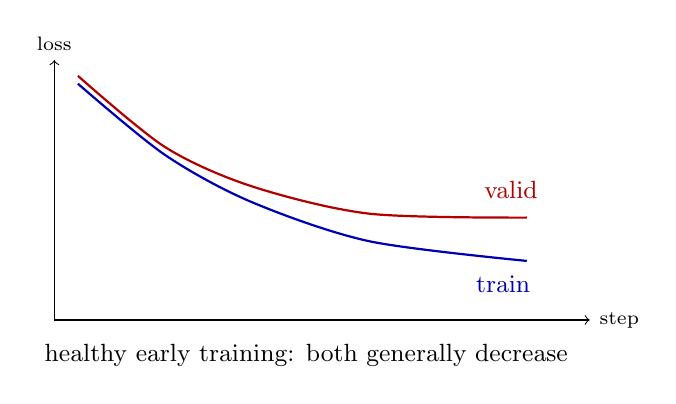
\begin{tikzpicture}[
  note/.style={font=\small, align=center}
]
\draw[->] (0,0) -- (6.8,0) node[right] {\scriptsize step};
\draw[->] (0,0) -- (0,3.3) node[above] {\scriptsize loss};
\draw[thick, blue!70!black] plot[smooth] coordinates {(0.3,3.0) (1.4,2.1) (2.5,1.5) (4.0,1.0) (6.0,0.75)};
\draw[thick, red!70!black] plot[smooth] coordinates {(0.3,3.1) (1.4,2.2) (2.5,1.7) (4.0,1.35) (6.0,1.3)};
\node[note, blue!70!black] at (5.7,0.45) {train};
\node[note, red!70!black] at (5.8,1.65) {valid};
\node[note] at (3.2,-0.45) {healthy early training: both generally decrease};
\end{tikzpicture}
\end{center}

Common patterns:

\begin{longtable}{p{0.32\textwidth}p{0.46\textwidth}}
\toprule
\term{Observation} & \term{Likely meaning} \\
\midrule
Train and validation loss decrease & learning is happening \\
Train decreases, validation rises & overfitting \\
Neither decreases & bug, bad learning rate, or data issue \\
Loss becomes NaN & numerical instability, too high LR, bad data, or precision issue \\
Loss is near \(\log V\) and flat & model may be guessing uniformly \\
\bottomrule
\end{longtable}

For TinyGPT with \(V=9\), uniform random guessing gives:

\[
\log(9)\approx2.197.
\]

If the initial loss is near this value, that can be normal. If it never moves, investigate.

\section{Case Study: A Successful GPT21 PyTorch Run}

Toy models teach the mechanism. A real run teaches the discipline. The GPT21
WikiText-103 DDP run on \texttt{wish01} gives us a concrete PyTorch reference point for
the rest of the book:

\begin{lstlisting}
run_name: gpt21-wikitext103-ddp
model: vocab_size 32000, block_size 512, layers 6, heads 6, n_embd 384
dtype: float16
train: micro_batch_size 1, gradient_accumulation_steps 32
optimizer: AdamW, lr 3e-4 -> 3e-5, warmup 300, weight_decay 0.1
checkpoint cadence: every 500 optimizer steps
final checkpoint: step-9999.pt and latest.pt
\end{lstlisting}

Assuming two DDP workers, the effective number of tokens per optimizer step is

\[
1 \times 2 \times 32 \times 512 = 32768.
\]

Across 10000 optimizer steps, the training loop therefore processes about

\[
32768 \times 10000 = 327{,}680{,}000
\]

token positions. This does not mean the dataset contains that many unique tokens. It
means the optimizer saw that many training positions, sampled from the token stream.

\begin{longtable}{p{0.20\textwidth}p{0.22\textwidth}p{0.22\textwidth}p{0.24\textwidth}}
\toprule
\term{Step} & \term{Train loss} & \term{Valid loss} & \term{Interpretation} \\
\midrule
750 & 5.4648 & 5.4842 & early learning, high perplexity \\
1500 & 4.7826 & 4.8514 & clear improvement \\
3000 & 4.2584 & 4.1988 & stable descent \\
5250 & 3.9644 & 3.7432 & validation has improved strongly \\
8250 & 3.8463 & 3.6265 & best listed validation point \\
9500 & 3.9707 & 3.6563 & still near best validation \\
9750 & 3.8039 & 3.8154 & final region, not perfectly monotonic \\
\bottomrule
\end{longtable}

The important pattern is not that every evaluation improves. It does not. With only
\texttt{eval\_iters = 20}, evaluation estimates are noisy. The professional conclusion is:

\begin{itemize}
  \item the run is successful because both train and validation loss move from about
  \(5.5\) toward the high \(3.x\) range;
  \item validation does not explode, so obvious overfitting is not the dominant story;
  \item the best listed validation loss, \(3.6265\), corresponds to perplexity
  \(e^{3.6265}\approx37.6\);
  \item the run should keep the best-validation checkpoint, not only the latest
  checkpoint;
  \item the same config and checkpoint set should become the PyTorch reference for
  Candle and llm.c comparisons.
\end{itemize}

This is the difference between a demo and an industry-useful training pack. A demo says,
``loss went down.'' A training pack says exactly which config, which data, which hardware,
which checkpoints, which metrics, and which backend produced the result.

\section{The One-Batch Overfit Test}

The most important beginner training test is:

\begin{quote}
Can the model overfit one tiny batch?
\end{quote}

Disable dropout, use a fixed batch, train for many steps, and expect loss to fall sharply.

\begin{center}
\begin{tikzpicture}[
  box/.style={draw, rounded corners=2pt, minimum height=0.62cm, text width=2.1cm, align=center},
  arrow/.style={-{Latex[length=2mm]}, thick}
]
\node[box, fill=blue!5] (fixed) at (0,0) {fixed batch};
\node[box, fill=yellow!18] (drop) at (2.7,0) {dropout = 0};
\node[box, fill=red!8] (train) at (5.4,0) {train many\\steps};
\node[box, fill=green!10] (loss) at (8.1,0) {loss should\\collapse};
\draw[arrow] (fixed) -- (drop);
\draw[arrow] (drop) -- (train);
\draw[arrow] (train) -- (loss);
\end{tikzpicture}
\end{center}

If one-batch loss does not fall:

\begin{itemize}
  \item check target shifting;
  \item check optimizer is receiving parameters;
  \item check \texttt{loss.backward()} and \texttt{optimizer.step()} are called;
  \item check model is in training mode;
  \item check logits and targets have correct shapes;
  \item check learning rate is not absurdly small or large.
\end{itemize}

\section{Engineering Practice}

Every training log should include:

\begin{itemize}
  \item step and tokens processed;
  \item train loss and validation loss;
  \item learning rate;
  \item gradient norm;
  \item throughput in tokens per second;
  \item batch size, accumulation steps, and world size;
  \item checkpoint path and config hash;
  \item model parameter count;
  \item hardware/device information.
\end{itemize}

Save enough state to resume:

\begin{itemize}
  \item model state dict;
  \item optimizer state dict;
  \item scheduler/training step;
  \item random seeds if reproducibility matters;
  \item config and tokenizer metadata.
\end{itemize}

\section{Hands-On Lab: Overfit One Batch}

Use TinyGPT with:

\begin{lstlisting}
vocab_size = 9
block_size = 5
n_layer = 2
n_head = 2
n_embd = 6
dropout = 0.0
\end{lstlisting}

Use one fixed batch:

\begin{lstlisting}[language=Python]
x = torch.tensor([[2, 3, 4, 5, 6],
                  [3, 4, 5, 6, 7]], dtype=torch.long)
y = torch.tensor([[3, 4, 5, 6, 7],
                  [4, 5, 6, 7, 8]], dtype=torch.long)
\end{lstlisting}

Training skeleton:

\begin{lstlisting}[language=Python]
model.train()
optimizer = torch.optim.AdamW(model.parameters(), lr=1e-2, weight_decay=0.0)

for step in range(300):
    logits, loss = model(x, y)
    optimizer.zero_grad(set_to_none=True)
    loss.backward()
    optimizer.step()

    if step % 25 == 0:
        print(step, loss.item())
\end{lstlisting}

Expected behavior: the loss should fall clearly. The exact value depends on initialization, but a tiny model should be able to memorize a tiny fixed batch.

\checkpoint

\begin{enumerate}
  \item Why do logits need softmax before they can be interpreted as probabilities?
  \item Why does cross entropy use \(-\log p_y\)?
  \item For softmax plus cross entropy, what is \(\partial \ell/\partial z_i\)?
  \item Why does training require more memory than inference?
  \item What is the difference between a parameter and an optimizer state tensor?
  \item Why does gradient accumulation divide the loss by \texttt{grad\_accum\_steps}?
  \item Why use learning-rate warmup?
  \item What does it mean if training loss falls while validation loss rises?
  \item Why is one-batch overfitting a useful debugging test?
  \item What should be saved to resume training faithfully?
\end{enumerate}

\subsection*{Solutions}

\begin{enumerate}
  \item Logits are unconstrained real scores. Softmax converts them into nonnegative values that sum to one.
  \item \(-\log p_y\) is small when the correct token probability is high and large when it is low, so it directly rewards assigning probability to the target.
  \item For one prediction, \(\partial \ell/\partial z_i=p_i-\mathbb{1}[i=y]\).
  \item Training must keep forward-pass information for backpropagation and store gradients. Inference only needs the forward computation.
  \item A parameter is a trainable model weight. Optimizer state is extra persistent information, such as AdamW moment estimates, used to update parameters.
  \item Dividing keeps the accumulated gradient scale similar to the gradient from one larger batch.
  \item Warmup avoids overly aggressive early updates when weights are random and gradients may be unstable.
  \item The model is overfitting: it is improving on training data while generalizing worse to held-out data.
  \item If a model cannot memorize one tiny batch, the training pipeline likely has a bug in data, targets, loss, gradients, optimizer, or mode.
  \item Save model weights, optimizer state, step/scheduler state, config, tokenizer metadata, and relevant reproducibility information.
\end{enumerate}
